\newpage
\section{Тестирование}
\label{sec:Testings}
В данном разделе представлены результаты функционального тестирования и экспериментов по исследованию эффективности разработанной программы.
\vspace{1.2em}

\subsection{Функциональное тестирование}

В ходе данного тестирования проверялось соответствие приложения
предъявленным функциональным требованиям. Тестирование приложения
проводилось вручную. В таблице~\ref{tab:тест} приведен протокол ручного тестирования основных аспектов работы системы.

\begin{table}[H]
    \setstretch{1.0}
    \caption{Функциональное тестирование приложения}
    \fontsize{12pt}{1em}\selectfont
    \vspace{1em}
    \begin{tabularx}{\linewidth}{|c|X|X|X|c|}
       \hline
        \textbf{№} & \textbf{Название теста} & \textbf{Действие} & \textbf{Ожидаемый результат} & \makecell{\textbf{Тест} \\ \textbf{пройден?}} \\ \hline
        1 & Проверка определения класса популярности. & На странице с вводом отправить данные и получить значение популярности. & Ранг популярности определен. & Да \\ \hline
        2 & Проверка прогнозирования звезд. & В форме на странице с вводом нажать на кнопку <<Определить>> и получить значение звезд. & Значение возможного количества звезд отображено.  & Да \\ \hline
        3 & Проверка ввода только численных значений. & На странице с вводом данных ввести значения, отличные от чисел. & В поля не вводятся не численные значения. & Да \\ \hline
        4 & Проверка отправки формы данных. & При незаполненных данных на странице ввода отправить форму. & Получено всплывающее уведомление, что поле не заполнено. & Да \\ \hline
        5 & Проверка выбора модели. & На главной странице выбрать <<Модель регрессии>> \ и отправить форму с выбранной моделью <<Случайный лес>>. & На странице результатов отображены результаты после прогнозирования с помощью модели <<Случайный лес>>. & Да \\ \hline
        \end{tabularx} 
    \label{tab:тест}
\end{table}
\vspace{1em}

\subsection{Вычислительные эксперименты}

\subsubsection*{Оценка моделей классификации с помощью метрик}

Метрики представляют собой инструменты оценки эффективности алгоритмов классификации, позволяющие оценить качество предсказаний модели на основе различных аспектов ее работы~\cite{manning2008introduction}. В данном разделе рассматриваются основные метрики, широко применяемые в задачах классификации.

\textit{Матрица ошибок} (Confusion Matrix) -- это таблица, используемая для оценки производительности модели классификации, позволяющая визуализировать результаты предсказаний по каждому классу. Она представляет собой матрицу, когда реальные значения классов из тестового набора данных сравниваются с предсказанными моделью. Основная матрица ошибок представлена в таблице~\ref{tabular:matrix}.

\begin{table}[h]
    \onehalfspacing \caption{Таблица матрицы ошибок}
    \fontsize{12pt}{1em}\selectfont
    \medskip
    \begin{tabularx}{\textwidth}{|X|X|X|} 
    \hline
        \backslashbox{}{}  & Positive & Negative \\ \hline
        Positive & True Positive (TP) & False Positive (FP)\\ \hline
        Negative & False Negative (FN) & True Negative (TN) \\ \hline
    \end{tabularx} 
    \label{tabular:matrix}
\end{table}
\vspace{1em}

В матрице ошибок присутствуют четыре основных термина: 

\begin{enumerateparendot}
    \item True Positive (TP) -- это количество объектов, которые модель верно предсказала как положительные (верно идентифицированные положительные классы).
    \item  True Negative (TN) -- это количество объектов, которые модель верно предсказала как отрицательные (верно идентифицированные отрицательные классы).
    \item  False Positive (FP) -- это количество объектов, которые модель неверно предсказала как положительные, хотя они на самом деле относятся к отрицательному классу (ложноположительные результаты).
    \item  False Negative (FN) -- это количество объектов, которые модель неверно предсказала как отрицательные, хотя они на самом деле относятся к положительному классу (ложноотрицательные результаты).
\end{enumerateparendot}

\textit{Аккуратность} (Accuracy) представляет собой долю правильных предсказаний модели относительно общего числа предсказаний. Она вычисляется по формуле~\ref{accuracy}.

\begin{equation}
\label{accuracy}
    Accuracy = \frac{TP + TN}{TP + TN + FP + FN} \ , 
\end{equation}
\vspace{0.3em}

где \( TP \) -- количество истинно положительных предсказаний, \( TN \) -- количество истинно отрицательных предсказаний, \( FP \) -- количество ложно положительных предсказаний и \( FN \) -- количество ложно отрицательных предсказаний.

\textit{Точность} (Precision) измеряет долю истинно положительных предсказаний среди всех предсказанных положительных случаев, в то время как \textit{полнота} (Recall) измеряет долю истинно положительных предсказаний среди всех истинно положительных случаев. Они вычисляются по~\ref{precision} и~\ref{recall}.

\begin{equation}
\label{precision}
    Precision = \frac{TP}{TP + FP} 
\end{equation}


\begin{equation}
\label{recall}
    Recall = \frac{TP}{TP + FN} 
\end{equation}
\vspace{1.5em}

\textit{F-мера} (F1-score) представляет собой гармоническое среднее между точностью и полнотой класса и является компромиссом между ними. Она вычисляется по формуле~\ref{f1}.

\begin{equation}
\label{f1}
F1 = \frac{2 \cdot Precision \cdot Recall}{Precision + Recall} 
\end{equation}
\vspace{1.5em}

Для каждой из моделей была составлена матрица ошибок, отражающая, какое количество элементов модель смогла верно определить относительно того класса популярности проекта, к которому она была определена ранее. На рисунке~\ref{ris:class} представлена матрица ошибок Градиентного бустинга, который показал хороший результат в сравнении с другими моделями. Для остальных рассмотренных в работе моделей были составлены аналогичные матрицы ошибок. Результаты представлены в~\hyperref[sec:matrix]{приложении Б}. 

\begin{figure}[h]
    \centering
    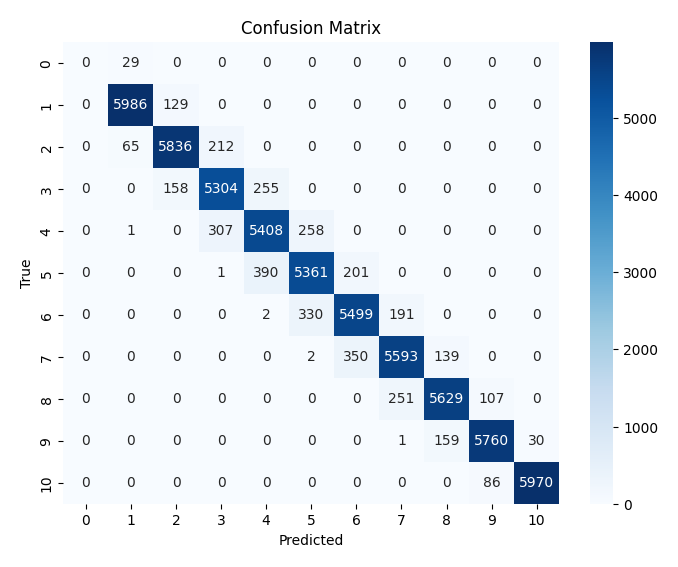
\includegraphics[width=1\linewidth]{pic/classification/gradient_boosting.png}
    \vspace{0.5em}\caption{Матрица ошибок Градиентного бустинга}
    \label{ris:class}
\end{figure}
\vspace{1em}

В рамках каждой модели есть свои параметры, которые влияют на обучение моделей, на точность определения проекта к классу популярности в зависимости от исходных параметров. Так, например, параметр n\_estimators указывает количество базовых моделей, которые будут объединены. Большее количество шагов может улучшить качество модели, но может увеличить время обучения. Значение random\_state управляет случайностью в модели. Задавая одно и то же значение, можно получить одинаковые результаты при каждом запуске обучения модели. В модели Градиентного бустинга есть параметр learning\_rate, контролирующий величину, на которую каждый базовый классификатор <<учится>> на ошибках предыдущих классификаторов.

Параметры помогают настроить модели таким образом, чтобы они давали оптимальные результаты для конкретного набора данных и задачи классификации. При этом изменение большинства параметров с целью улучшения точности ведет к значительному увеличению времени обучения модели. Время обучения тоже является важным критерием при выборе модели и параметров. 

В результате необходимо найти подходящее соотношение времени обучения и результатов метрик, для этого было проведено сравнение скорости обучения модели и результатов значений метрик на разных значениях параметра n\_estimators. На рисунке~\ref{ris:graph} представлен график зависимости времени обучения модели и результат значений метрик, где видно, что увеличение параметра начало все меньше влиять на значения метрик, при этом время выполнения также растет, поэтому оптимально искать среднее значение. Для других моделей с хорошими показателями метрик были составлены аналогичные графики зависимостей. Результаты представлены в \hyperref[sec:graphics]{приложении В}. 

\begin{figure}[h]
    \centering
    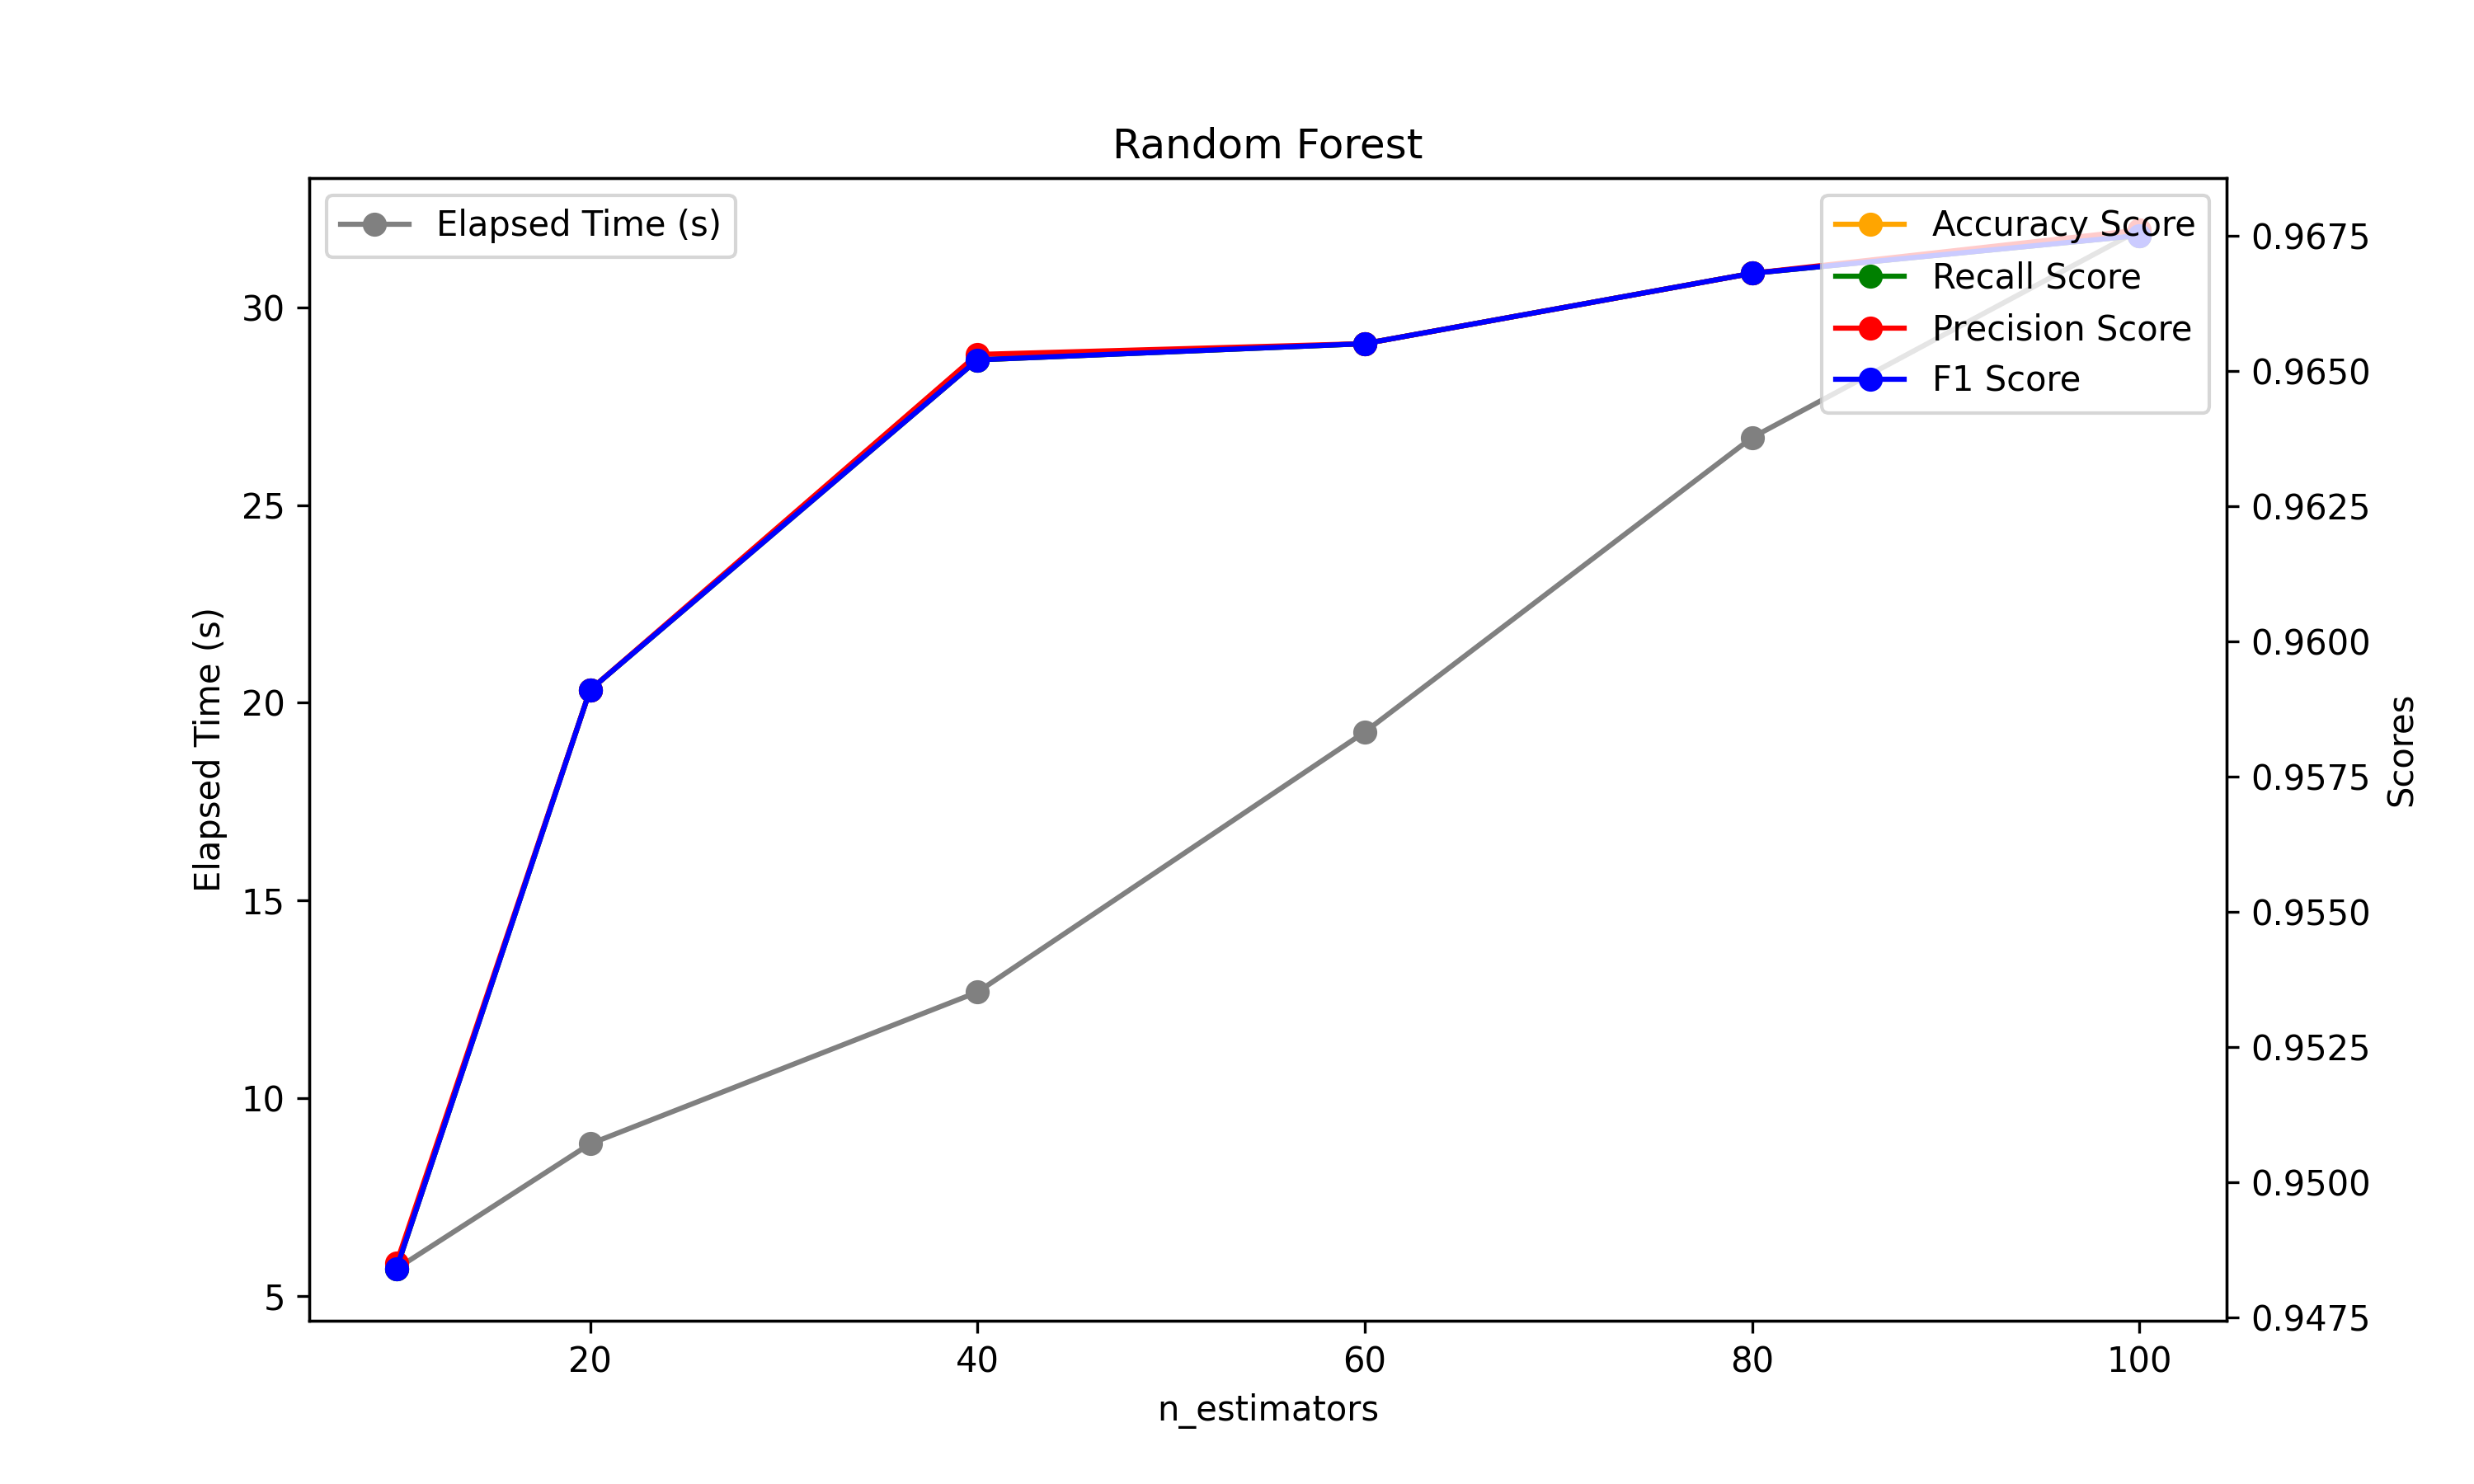
\includegraphics[width=1\linewidth]{pic/statistic/random_forest.png}
    \vspace{-0.5em}\caption{График зависимости времени и метрик Случайного леса}
    \label{ris:graph}
\end{figure}
\vspace{1em}

После определения оптимальных значений в параметрах и оценке их времени выполнения в каждой модели было выполнено обучение и вычисление значений метрик. Результаты рассчитанных метрик для реализованных моделей классификации представлены в таблице~\ref{tabular:table-classification}. Чем ближе значение к 1, тем более точно модель способна определить класс.

\begin{table}[h]
    \onehalfspacing \caption{Метрики задач классификации}
    \fontsize{12pt}{1em}\selectfont
    \medskip
        \begin{tabularx}{\textwidth}{|l|>{\centering\arraybackslash}X|>{\centering\arraybackslash}X|>{\centering\arraybackslash}X|>{\centering\arraybackslash}X|}
        \hline
        \backslashbox{}{}  & accuracy & precision & recall & F-score \\ \hline
            Decision Tree & 0.9414 & 0.9415 & 0.9413 & 0.9415 \\  \hline 
            Random Forest & 0.9457 & 0.9675 & 0.9674 & 0.9675 \\  \hline 
            Gradient Boosting & 0.7608 & 0.7731 & 0.7602 & 0.7628 \\  \hline 
            AdaBoosting & 0.5643 & 0.4362 & 0.6698 & 0.4596 \\  \hline 
            Naive Bayes & 0.7346 & 0.6258 & 0.6387 & 0.6273 \\  \hline 
        \end{tabularx}
    \label{tabular:table-classification}
\end{table}
\vspace{1.5em}

\subsubsection*{Оценка моделей регрессии с помощью метрик}

Метрики в задачах регрессии играют важную роль в оценке точности и эффективности модели. Они позволяют оценить, насколько хорошо модель соответствует реальным данным и насколько точны ее прогнозы. В данном разделе рассматриваются основные метрики, применяемые для оценки моделей регрессии.

\textit{Средняя абсолютная ошибка} (Mean Absolute Error, MAE) представляет собой среднее абсолютное значение разницы между фактическими значениями и прогнозируемыми значениями модели. Она вычисляется по формуле~\ref{mae}.

\begin{equation}
\label{mae}
    MAE = \frac{1}{n} \sum_{i=1}^{n} |y_i - \hat{y}_i|  \ ,
\end{equation}
\vspace{0.3em}

где \( y_i \) -- фактическое значение, \( \hat{y}_i \) -- прогнозное значение, а \( n \) -- количество наблюдений.
\vspace{1em}

\textit{Среднеквадратичная ошибка} (Mean Squared Error, MSE) измеряет среднеквадратичную разницу между фактическими значениями и прогнозируемыми значениями модели. Она вычисляется по формуле~\ref{mse}.

\begin{equation}
\label{mse}
    MSE = \frac{1}{n} \sum_{i=1}^{n} (y_i - \hat{y}_i)^2 \ ,
\end{equation}
\vspace{0.3em}

где \( y_i \) -- фактическое значение, \( \hat{y}_i \) -- прогнозное значение, а \( n \) --количество наблюдений.
\vspace{1em}

\textit{Коэффициент детерминации} (Coefficient of Determination, \( R^2 \)) измеряет пропорцию вариации зависимой переменной, объясненной моделью, к общей вариации зависимой переменной. Он принимает значения от 0 до 1 и чем ближе значение \( R^2 \) к 1, тем лучше модель соответствует данным. \( R^2 \) вычисляется по формуле~\ref{r2}.

\begin{equation}
\label{r2}
R^2 = 1 - \frac{\sum_{i=1}^{n} (y_i - \hat{y}_i)^2}{\sum_{i=1}^{n} (y_i - \bar{y})^2} \ ,
\end{equation}
\vspace{0.3em}

где \( \bar{y} \) -- среднее значение зависимой переменной. 

\vspace{1em}

Эти метрики предоставляют информацию о точности и качестве модели регрессии, помогая исследователям и практикам принимать информированные решения на основе результатов их работы.

Аналогично моделям классификации были определены оптимальные значения в параметрах. Результаты рассчитанных метрик для реализованных моделей регрессии представлены в таблице~\ref{tabular:table-regression}.

\begin{table}[h]
    \onehalfspacing \caption{Метрики задач регрессии}
    \fontsize{12pt}{1em}\selectfont
    \medskip
        \begin{tabularx}{\textwidth}{|l|>{\centering\arraybackslash}X|>{\centering\arraybackslash}X|>{\centering\arraybackslash}X|}
        \hline
            \backslashbox{}{}  & MSE & MAE & $R^2$ \\ \hline
            Decision Tree & 97601.26 & 466.59 & 0.2150 \\  \hline 
            Random Forest & 54962.27 & 355.25 & 0.5580 \\  \hline 
            Gradient Boosting & 55149.55 & 367.19 & 0.5563 \\  \hline 
            Linear Regression & 70683.04 & 530.50 &  0.4317 \\  \hline 
        \end{tabularx}
    \label{tabular:table-regression}
\end{table}